\input{../../v3_rp/preamble}
\usepackage{longtable}
\usepackage{array}
\graphicspath{{../../}}
\makeatletter\def\input@path{{./}{../../}{../../v3_rp/}}\makeatother
\title{\bfseries Where Being Early Costs and Being Unusual Pays\\
\large A summary by industry and by persistence}
\author{Eric Silver}
\date{Working document, September 2026}

\begin{document}
\maketitle

\noindent Every US trademark filing is scored on two positions of its
goods-and-services language within its industry (Nice class)
\citep{SilverCorpus2026}. \emph{Atypicality} is how unusual the
language is against both the filings that came before and those that
came after. \emph{Lead} is whether later filings moved toward it: a
leading filing described a kind of offering that became more common after
it was filed. The outcomes are the five-year proof that a registered
mark's goods are still sold, the ten-year renewal among marks that passed
the proof, and the capital-markets record of the owner.

\section*{The headline: unusual language pays after registration; early
language costs}

\emph{The two positions pull in opposite directions at every stage.}
Among first-time filers, one standard deviation of atypicality lowers the
chance of registration by 1.0 point and raises the chance of passing the
five-year proof by 1.3 and of renewal by 1.4. One standard deviation of
lead raises the chance of registration by 0.5 point and lowers the chance
of passing the proof by 1.0 and of renewal by 0.4. Unusual language is
harder to register and more durable once registered; early language is
easier to register and less durable.

\begin{center}\small
\begin{tabular}{lrr}
\toprule
Stage (first-time filers; points per SD) & Atypicality & Lead \\
\midrule
Registered (of all filed) & $-0.98$ & $+0.47$ \\
Passed the five-year proof (of registered) & $+1.31$ & $-0.97$ \\
Renewed at year ten (of those that passed) & $+1.38$ & $-0.43$ \\
Filed any private-offering notice (of registered) & $-0.17$ & $-0.32$ \\
Listed after the round (of funded) & $+0.87$ & $-0.53$ \\
\bottomrule
\end{tabular}
\end{center}

\emph{Across all registrations, the most unusual filing in a class and
year survives the proof 4.6 points more often than the most typical, and
the most leading 1.6 points less often than the most lagging.} Among
marks that passed the proof, the same comparisons at renewal are $+3.7$
and $-0.7$. Both effects persist past the first test; the benefit of
atypicality persists more fully than the cost of lead.

\section*{By industry: where the cost of leading falls}

\emph{Where leading costs at the proof, it also costs at renewal.} Across
Nice classes the lead effect at the proof and the lead effect at renewal
correlate at 0.67; for atypicality the correlation is 0.74. Industries
differ in a stable way, not by chance at one test (Figure~1).

\emph{In twelve classes the penalty persists through both tests.} The
largest are tobacco and vaping (class 34: $-11.3$ points at the proof,
$-7.9$ at renewal), technology and science services (42: $-9.6$,
$-7.9$), medical devices (10: $-7.2$, $-4.8$), meat and dairy (29:
$-6.5$, $-4.9$), lighting and heating (11: $-5.9$, $-6.1$), hand tools
(8: $-5.4$, $-4.1$) and fabrics (24: $-4.0$, $-6.0$).

\emph{In five classes the penalty is confined to the proof.} Electronics
and software (9: $-3.4$ at the proof, $+1.0$ at renewal), advertising and
business services (35: $-3.0$, $+0.7$), hotels and restaurants (43:
$-3.6$, $+0.6$), chemicals (1: $-2.2$, $-0.3$) and clothing (25: $-2.0$,
$+0.9$): leading filings that clear the first test are no more likely
than lagging ones to be abandoned afterwards. In these classes the cost
of leading is paid at the first test.

\emph{In four classes the penalty appears only at renewal.} Education
and entertainment (41: 0.0 at the proof, $-3.6$ at renewal), housewares
(21: 0.0, $-4.0$), jewelry (14: $-1.9$, $-4.6$) and fuels (4: $-1.8$,
$-5.8$).

\emph{In five classes leading is rewarded at both tests.} Construction
and repair (37: $+4.0$, $+4.5$), transport and storage (39: $+4.5$,
$+3.2$), toys and sporting goods (28: $+3.7$, $+2.4$), firearms (13:
$+2.6$, $+3.9$) and treatment of materials (40: $+1.7$, $+4.7$).

\emph{In three the reward is confined to the proof.} Beer and soft drinks
(32: $+9.6$ at the proof, $-0.1$ at renewal), paints (2: $+4.7$, $+0.8$)
and legal and personal services (45: $+2.4$, $-1.6$). Beer's reward
belongs to the 2010s: the class's leading language was beer, beer
registrations went from a third of the class to two-thirds, and leading
beer filings passed the proof 10 points more often than lagging ones;
at renewal, leading neither helped nor hurt.

\emph{Tobacco's penalty is a product change, not a property of the
industry.} The class-34 penalty is confined to registrations of 2013--18
($-23.4$ points; $+4.1$ and $+0.5$ in the two earlier periods), when
e-cigarette and vaping language went from none of the class's
registrations to 46\%. Vaping registrations pass the proof 15.8 points
less often than the class's others, and within each product ---
vaping, cigars, cigarettes, hookah --- leading is not penalized. The
class-level penalty is between products: in class 34, leading language
meant vaping, and vaping marks were abandoned.

\emph{Grouped, the three kinds of class are stable over time.} In the
group where leading costs most, the penalty at the proof is $-5.4$,
$-7.5$ and $-6.7$ points in registrations of 2002--07, 2008--12 and
2013--18, and $-4.7$ at renewal. In the middle group it moves from $+1.0$
to $-1.6$. In the group where leading costs least, the reward is
concentrated in 2013--18 ($+9.7$) and does not carry to renewal; its
survival curve is an inverted U, highest near the 65th percentile of lead
and lower at both ends.

\section*{By industry: where unusual language pays}

\emph{Atypicality pays most in large, technical and service classes and
costs in several manufacturing and trade classes.} The most unusual
filings survive the proof much more often than the most typical in
electronics and software (9: $+16$ points; $+14$ at renewal), advertising
and business services (35: $+13$; $+9$), fuels (4: $+12$), telecommunications
(38: $+10$; $+12$), pharmaceuticals (5: $+11$; $+8$) and cosmetics (3: $+8$;
$+11$). They survive less often in machinery (7: $-11$; $-9$), legal and
personal services (45: $-7$; $-5$), chemicals (1: $-5$; $-4$) and paints
(2: $-5$; $-4$), and at renewal in hotels and restaurants (43: $-6$) and
beer (32: $-6$).

\emph{Where leading pays, unusual language costs.} In the group where
leading costs least, the most unusual filings pass the proof 2.9 points
less often than the most typical; in the group where leading costs most,
atypicality has no effect ($+0.7$); in the large middle group it is worth
5.8 points. The industries that reward the early mover reward the
conventional description of what it sells.

\section*{The hypotheses: who, what, when}

\emph{Resources: counsel removes most of the cost of leading at the proof
and part of it at renewal} \citep{LiebermanMontgomery1998}. Counsel is
worth 19.4 points of survival at the proof and 14.6 at renewal. It
changes the lead effect by $+5.0$ points at the proof and $+2.2$ at
renewal. Among self-filed registrations leading costs about 5.5 points
at the proof and 2.6 at renewal; among counsel-represented ones, about
0.5 and 0.4.

\emph{Network effects: platforms pay for leading at both tests}
\citep{LiebermanMontgomery1988}. Platform and network offerings survive
the proof 8.2 points less often, and leading costs them 7.9 points more
than it costs other filings at the proof and 8.5 points more at
renewal. This is the most persistent penalty the record shows, and the
reverse of the network-effects prediction.

\emph{General-purpose technologies: the extra cost of leading is paid at
the proof.} Filings using internet, mobile, cloud, social-media, AI or
blockchain vocabulary pay 2.9 points more for leading at the proof and
0.6 (not distinguishable from zero) at renewal.

\emph{Pace of change: leading costs most where markets grow fast}
\citep{SuarezLanzolla2007}. With the time trend held, leading costs 4.7
points where the class's theme mix and filing volume both change fast,
2.7 where only volume grows, 1.0 in calm class-years and 0.8 where only
the mix turns over, the reverse of the ordering the pace-of-change
account predicts.

\emph{Time: the cost of leading has grown.} The penalty at the proof is
$-0.1$ points for registrations of 2002--07 and $-2.2$ and $-2.0$ for
2008--12 and 2013--18, about 0.8 points more every five years; the
benefit of atypicality has fallen from 5.9 to 3.9. Booms (1998--2000,
2005--07) and busts (2001--02, 2008--09) do not differ from other years
once the trend is held.

\emph{Order of entry: pioneers and early followers fail alike}
\citep{GolderTellis1993}. Filings using a new product vocabulary in its
first two years in a class fail the proof 12.8 points more often than
their class and year; filings two to five years in, 11.8 points more
often. Pioneers fail, and early followers fail at the same rate.

\emph{Complementary assets: in consumer packaged goods the cost falls on
incumbents} \citep{Teece1986}. Leading costs established owners (25 or
more earlier filings) 4.9 points and first-time filers nothing.

\emph{Uncontested market space: the exemplars did not lead}
\citep{KimMauborgne2004}. The registrations of [yellow tail]'s owner,
Cirque du Soleil, Southwest Airlines, NetJets, Accor, Starbucks and Home
Depot sit in the middle of their classes' lead distributions; only
Curves's lean leading. Themes imported from another class survive more
often (2.0 points) and pay the same for leading.

\emph{Geography: clustering lowers survival but does not change the cost
of leading.} A co-location measure that allows several hubs identifies
Santa Clara for semiconductors and New York, San Francisco and Los
Angeles for social networking. A theme's co-location lowers survival by
1.6 points per SD; filers inside a hub pay the same for leading as
filers outside.

\section*{What the record says about being early}

The cost of being early is not general. It is large and lasting in a
dozen classes, from tobacco and technology services to medical devices
and meat and dairy, and in platforms; it is paid once, at the first
test, in electronics and software, advertising, hotels and restaurants
and clothing, and in general-purpose-technology vocabulary; it is nearly
absent where counsel is retained; and it turns into a reward in construction, transport, toys
and firearms, and, for a decade, in beer. Unusual language is rewarded in
most classes and at both tests, except in the classes that reward the
early mover, where the conventional description survives.

\begin{figure}[htbp]
\centering
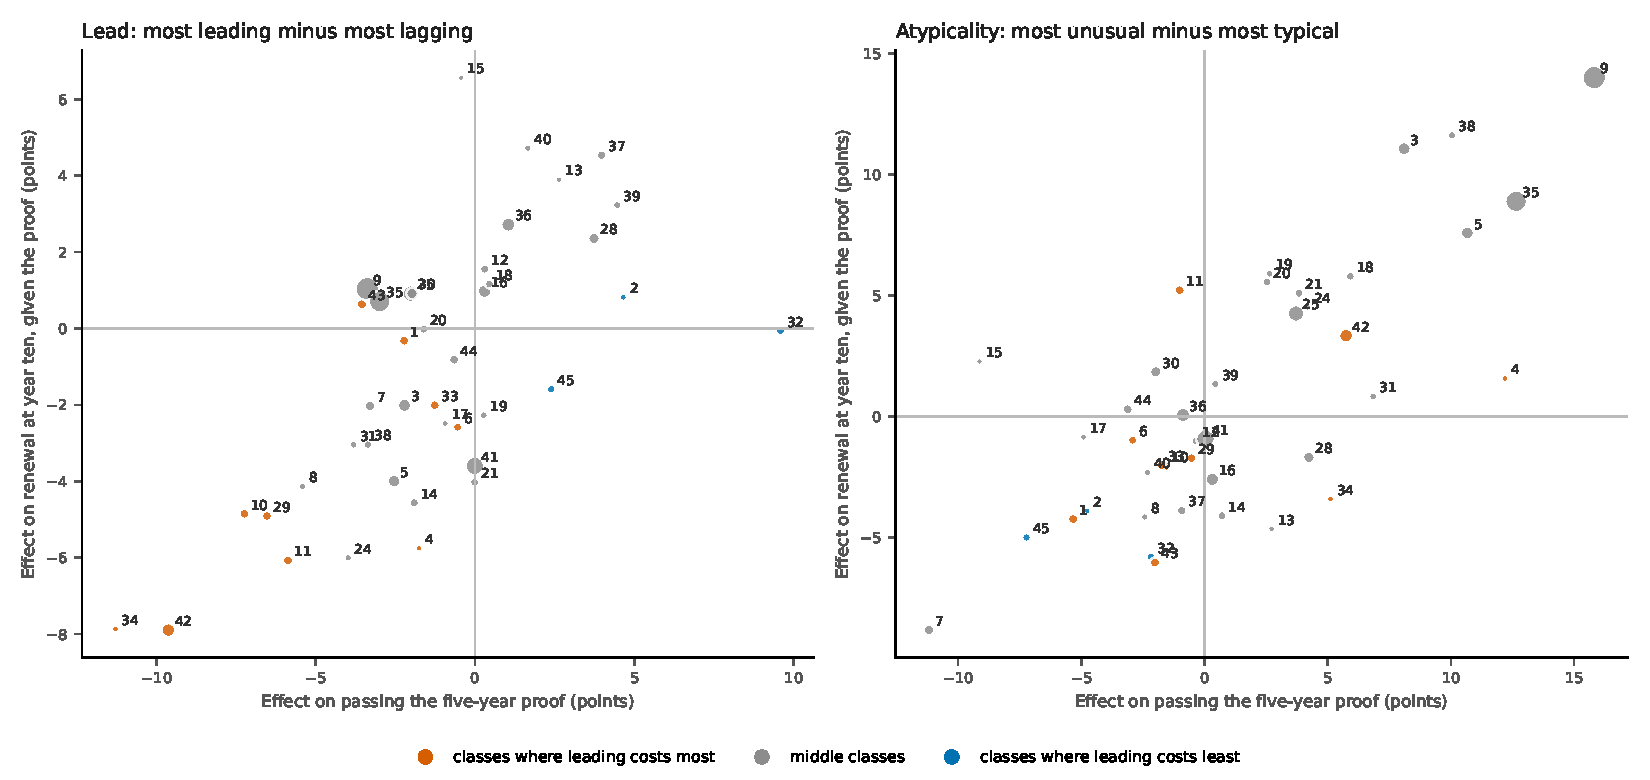
\includegraphics[width=\textwidth]{figures/fig_persistence.pdf}
\caption{Lead and atypicality effects by Nice class at the five-year
proof ($x$) and at renewal among marks that passed the proof ($y$).
Points are classes, sized by registrations and coloured by the class
groups formed from lead effects on half of owners. Effects are the
survival difference, in percentage points, between the top and bottom of
the class-and-year distribution, with class $\times$ registration-year
fixed effects and the paper's controls.}
\end{figure}

\section*{Appendix: every class}

Lead and atypicality effects by class (percentage points, top minus
bottom of the class-and-year distribution; standard errors in
parentheses for lead). A class is placed in a lead pattern when its
effect at a test is at least 2 points (1.5 for persistent benefits);
registrations 2002--18 for the proof and 2002--13, among those that
passed, for renewal.

{\small\begin{longtable}{r>{\raggedright\arraybackslash}p{3.7cm}rrrrr}
\toprule & & & \multicolumn{2}{c}{Lead} & \multicolumn{2}{c}{Atypicality} \\ \cmidrule(lr){4-5}\cmidrule(l){6-7} Class & & Registrations & Proof & Renewal & Proof & Renewal \\ \midrule \endhead
\addlinespace\multicolumn{7}{l}{\emph{Lead: penalty persists}} \\
34 & Tobacco, vaping & 13,993 & $-$11.3 (2.8) & $-$7.9 (4.5) & +5.1 & $-$3.4 \\
42 & Technology, science services & 127,407 & $-$9.6 (0.6) & $-$7.9 (1.1) & +5.7 & +3.3 \\
10 & Medical devices & 55,537 & $-$7.2 (1.0) & $-$4.8 (1.5) & $-$1.6 & $-$2.1 \\
29 & Meat, dairy, processed & 55,503 & $-$6.5 (1.2) & $-$4.9 (1.8) & $-$0.5 & $-$1.7 \\
11 & Lighting, heating & 55,383 & $-$5.9 (1.1) & $-$6.1 (1.7) & $-$1.0 & +5.2 \\
8 & Hand tools & 19,542 & $-$5.4 (1.6) & $-$4.1 (2.6) & $-$2.4 & $-$4.2 \\
24 & Fabrics & 18,531 & $-$4.0 (1.8) & $-$6.0 (2.9) & +4.2 & +4.5 \\
31 & Agricultural produce & 25,317 & $-$3.8 (1.8) & $-$3.0 (2.7) & +6.8 & +0.8 \\
38 & Telecommunications & 32,421 & $-$3.4 (1.3) & $-$3.0 (2.2) & +10.0 & +11.6 \\
7 & Machinery & 66,181 & $-$3.3 (1.0) & $-$2.0 (1.3) & $-$11.2 & $-$8.8 \\
5 & Pharmaceuticals & 108,181 & $-$2.5 (1.4) & $-$4.0 (1.2) & +10.7 & +7.6 \\
3 & Cosmetics, cleaning & 113,917 & $-$2.2 (0.9) & $-$2.0 (1.4) & +8.1 & +11.1 \\
\addlinespace\multicolumn{7}{l}{\emph{Lead: penalty appears late}} \\
14 & Jewelry & 45,289 & $-$1.9 (1.0) & $-$4.6 (2.0) & +0.7 & $-$4.1 \\
4 & Lubricants, fuels & 11,780 & $-$1.8 (2.6) & $-$5.8 (3.8) & +12.2 & +1.6 \\
21 & Housewares & 40,927 & 0.0 (1.2) & $-$4.0 (1.9) & +3.8 & +5.1 \\
41 & Education, entertainment & 254,579 & 0.0 (0.5) & $-$3.6 (0.8) & 0.0 & $-$0.9 \\
\addlinespace\multicolumn{7}{l}{\emph{Lead: penalty fades}} \\
43 & Hotels, restaurants & 60,493 & $-$3.6 (0.9) & +0.6 (1.6) & $-$2.0 & $-$6.0 \\
9 & Electronics, software & 426,177 & $-$3.4 (0.5) & +1.0 (0.7) & +15.8 & +14.0 \\
35 & Advertising, business & 353,547 & $-$3.0 (0.4) & +0.7 (0.7) & +12.6 & +8.9 \\
1 & Chemicals & 55,166 & $-$2.2 (1.0) & $-$0.3 (1.4) & $-$5.3 & $-$4.2 \\
25 & Clothing & 197,259 & $-$2.0 (0.5) & +0.9 (0.9) & +3.7 & +4.3 \\
\addlinespace\multicolumn{7}{l}{\emph{Lead: benefit persists}} \\
40 & Treatment of materials & 19,797 & +1.7 (1.5) & +4.7 (2.5) & $-$2.3 & $-$2.3 \\
13 & Firearms & 8,387 & +2.6 (2.6) & +3.9 (4.2) & +2.7 & $-$4.6 \\
28 & Toys, sporting goods & 82,356 & +3.7 (1.9) & +2.4 (1.9) & +4.2 & $-$1.7 \\
37 & Construction, repair & 49,178 & +4.0 (1.0) & +4.5 (1.6) & $-$0.9 & $-$3.9 \\
39 & Transport, storage & 30,844 & +4.5 (1.3) & +3.2 (2.1) & +0.4 & +1.3 \\
\addlinespace\multicolumn{7}{l}{\emph{Lead: benefit fades}} \\
45 & Legal, personal services & 34,032 & +2.4 (1.1) & $-$1.6 (2.4) & $-$7.2 & $-$5.0 \\
2 & Paints & 13,215 & +4.7 (2.0) & +0.8 (3.2) & $-$4.8 & $-$3.9 \\
32 & Beer, soft drinks & 37,724 & +9.6 (1.3) & $-$0.1 (2.7) & $-$2.2 & $-$5.8 \\
\addlinespace\multicolumn{7}{l}{\emph{Lead: small}} \\
30 & Coffee, bakery, staples & 79,726 & $-$2.0 (0.9) & +0.9 (1.5) & $-$2.0 & +1.8 \\
20 & Furniture & 43,033 & $-$1.6 (1.1) & 0.0 (1.9) & +2.5 & +5.6 \\
33 & Wine, spirits & 52,838 & $-$1.3 (1.2) & $-$2.0 (2.0) & $-$1.7 & $-$2.0 \\
17 & Rubber, plastics & 14,684 & $-$0.9 (1.7) & $-$2.5 (2.5) & $-$4.9 & $-$0.9 \\
44 & Medical, beauty services & 56,969 & $-$0.7 (0.9) & $-$0.8 (1.7) & $-$3.1 & +0.3 \\
6 & Metal goods & 41,413 & $-$0.5 (1.0) & $-$2.6 (1.5) & $-$2.9 & $-$1.0 \\
15 & Musical instruments & 6,486 & $-$0.4 (2.6) & +6.6 (3.9) & $-$9.1 & +2.3 \\
19 & Building materials & 25,319 & +0.3 (1.5) & $-$2.3 (2.1) & +2.6 & +5.9 \\
16 & Paper, printed matter & 126,216 & +0.3 (0.7) & +1.0 (1.0) & +0.3 & $-$2.6 \\
12 & Vehicles & 43,416 & +0.3 (1.2) & +1.6 (1.7) & $-$0.3 & $-$1.0 \\
18 & Leather goods & 39,283 & +0.4 (1.1) & +1.2 (2.1) & +5.9 & +5.8 \\
36 & Insurance, finance & 141,201 & +1.0 (0.7) & +2.7 (1.1) & $-$0.9 & +0.1 \\
\bottomrule\end{longtable}}


\begin{thebibliography}{99}

\bibitem[Golder \& Tellis(1993)]{GolderTellis1993}
Golder, P.~N., \& Tellis, G.~J. (1993). Pioneer advantage: Marketing logic or
marketing legend? \emph{Journal of Marketing Research}, 30(2), 158--170.

\bibitem[Kim \& Mauborgne(2004)]{KimMauborgne2004}
Kim, W.~C., \& Mauborgne, R. (2004). Blue ocean strategy. \emph{Harvard
Business Review}, 82(10), 76--84.

\bibitem[Lieberman \& Montgomery(1988)]{LiebermanMontgomery1988}
Lieberman, M.~B., \& Montgomery, D.~B. (1988). First-mover advantages.
\emph{Strategic Management Journal}, 9(S1), 41--58.

\bibitem[Lieberman \& Montgomery(1998)]{LiebermanMontgomery1998}
Lieberman, M.~B., \& Montgomery, D.~B. (1998). First-mover (dis)advantages:
Retrospective and link with the resource-based view. \emph{Strategic
Management Journal}, 19(12), 1111--1125.

\bibitem[Silver(2026)]{SilverCorpus2026}
Silver, E. (2026). An event-dated corpus of US trademark prosecution and
a two-sided measure of vocabulary position. SSRN Working Paper 7520758.
\url{https://ssrn.com/abstract=7520758}.

\bibitem[Su\'arez \& Lanzolla(2007)]{SuarezLanzolla2007}
Su\'arez, F.~F., \& Lanzolla, G. (2007). The role of environmental
dynamics in building a first mover advantage theory. \emph{Academy of
Management Review}, 32(2), 377--392.

\bibitem[Teece(1986)]{Teece1986}
Teece, D.~J. (1986). Profiting from technological innovation:
Implications for integration, collaboration, licensing and public
policy. \emph{Research Policy}, 15(6), 285--305.

\end{thebibliography}

\end{document}
